% Scientific Paper: AI-Augmented Virtual Tumor Board with Progressive Disclosure Visualization
% Adapted for HCI/Human Factors in Oncology Decision Support

\documentclass[11pt,twocolumn]{article}

% Packages
\usepackage[utf8]{inputenc}
\usepackage[T1]{fontenc}
\usepackage{amsmath,amssymb}
\usepackage{graphicx}
\usepackage{booktabs}
\usepackage{hyperref}
\usepackage{xcolor}
\usepackage{tikz}
\usetikzlibrary{shapes.geometric, arrows, positioning, fit, backgrounds, calc}
\usepackage{float}
\usepackage{algorithm}
\usepackage{algpseudocode}
\usepackage{listings}
\usepackage{enumitem}
\usepackage{caption}
\usepackage{subcaption}
\usepackage{geometry}
\geometry{margin=1in}

% Custom colors
\definecolor{emerald}{RGB}{16,185,129}
\definecolor{skyblue}{RGB}{59,130,246}
\definecolor{amber}{RGB}{245,158,11}
\definecolor{rose}{RGB}{244,63,94}
\definecolor{slate}{RGB}{71,85,105}

% Title
\title{%
\textbf{AI-Augmented Virtual Tumor Board with Progressive Disclosure Visualization for Disease Progression Monitoring} \\[0.5em]
\large A Human-Centered Design Approach to Reduce Cognitive Load in Oncology Decision Support
}

\author{
Virtual Tumor Board Development Team \\
Open Source Oncology AI Initiative \\
\texttt{github.com/oss-virtual-tumor-board}
}

\date{January 2026}

\begin{document}

\maketitle

% Abstract
\begin{abstract}
Tumor board meetings are essential for multidisciplinary cancer care, yet preparation is time-consuming and cognitive demands are high across diverse stakeholders---from patients to subspecialist oncologists. We present an open-source AI-augmented Virtual Tumor Board (VTB) system that integrates multi-agent deliberation with a novel progressive disclosure visualization framework for disease progression monitoring. Our system employs seven specialized AI agents (surgical oncology, medical oncology, radiation oncology, radiology, pathology, genetics, and palliative care) orchestrated through a structured ``Chain of Debate'' mechanism grounded in society-specific clinical guidelines via retrieval-augmented generation (RAG). Central to our contribution is a human-centered visualization system that adapts disease progression displays across four expertise levels: patients/caregivers, non-oncologist clinicians, oncologists, and radiology specialists. Following established Human-Computer Interaction (HCI) principles---including progressive disclosure, Gestalt grouping, and semantic color mapping---our visualizations reduce cognitive load while maintaining clinical accuracy. We demonstrate RECIST 1.1 calculation, longitudinal lesion tracking, and interactive charting modalities including waterfall plots, swimmer plots, spider diagrams, and anatomical heat maps. The system integrates Google MedGemma for medical image analysis, supporting both DICOM uploads and phone-captured imaging for resource-limited settings. This paper details the system architecture, visualization design rationale, implementation, and discusses implications for democratizing access to expert oncology decision support.
\end{abstract}

% Keywords
\noindent\textbf{Keywords:} Tumor Board, Multi-Agent Systems, Medical Visualization, Progressive Disclosure, RECIST, MedGemma, Human-Centered Design, Cognitive Load, Oncology Decision Support

\section{Introduction}

\subsection{Background and Motivation}

Multidisciplinary tumor boards (MTBs) represent the gold standard for cancer treatment planning, bringing together specialists from surgery, medical oncology, radiation oncology, radiology, pathology, genetics, and palliative care \cite{navify2024}. However, several challenges limit their effectiveness and accessibility:

\begin{enumerate}[leftmargin=*]
    \item \textbf{Preparation burden}: Case preparation averages 47 minutes per complex case, limiting throughput
    \item \textbf{Access inequality}: Many patients, particularly in resource-limited settings, lack access to comprehensive tumor boards
    \item \textbf{Cognitive overload}: Clinicians must synthesize imaging, pathology, genomics, and treatment literature simultaneously
    \item \textbf{Communication gaps}: Information must be conveyed to stakeholders with vastly different expertise levels
\end{enumerate}

Recent advances in large language models (LLMs) and vision-language models offer opportunities to address these challenges. Microsoft's MAI-DxO demonstrated that multi-agent orchestration can improve diagnostic accuracy through structured deliberation \cite{maidxo2025}. Similarly, Google's MedGemma provides state-of-the-art medical image interpretation capabilities \cite{medgemma2025}.

\subsection{Contributions}

This paper makes the following contributions:

\begin{enumerate}[leftmargin=*]
    \item A \textbf{multi-agent architecture} for oncology tumor board simulation, adapting MAI-DxO's diagnostic orchestrator to treatment planning with seven specialty-specific agents
    
    \item A \textbf{progressive disclosure visualization framework} for disease progression that adapts complexity to four expertise levels, following HCI best practices for cognitive load reduction
    
    \item Integration of \textbf{MedGemma} for medical image analysis with support for both DICOM and phone-captured imaging
    
    \item A complete \textbf{RECIST 1.1 implementation} with interactive measurement tracking and response visualization
    
    \item An \textbf{open-source implementation} designed for deployment in resource-limited healthcare settings
\end{enumerate}

\section{Related Work}

\subsection{AI in Tumor Board Support}

Commercial solutions like Roche's NAVIFY Clinical Hub provide tumor board workflow management with guideline integration and clinical trial matching \cite{navify2024}. However, these systems lack AI-driven deliberation capabilities and are cost-prohibitive for many institutions.

Academic efforts have explored natural language processing for tumor board documentation \cite{nlptb2023} and machine learning for treatment recommendation \cite{mlonc2024}, but few have addressed the visualization challenges for diverse stakeholders.

\subsection{Multi-Agent Medical AI}

The MAI-DxO system \cite{maidxo2025} demonstrated that multiple AI ``physicians'' with distinct roles (hypothesis generation, test selection, challenging assumptions) improve diagnostic accuracy. Our work extends this paradigm to treatment planning with oncology-specific agent personas grounded in society guidelines.

\subsection{Medical Visualization and HCI}

Effective medical visualization requires careful attention to cognitive load \cite{cogload2020}. Saloni Dattani's visualization principles emphasize clarity over simplicity, direct labeling, semantic color mapping, and progressive disclosure \cite{saloni2025}. These principles inform our multi-level visualization framework.

\section{System Architecture}

\subsection{High-Level Overview}

Figure \ref{fig:architecture} presents the system architecture. The Virtual Tumor Board comprises three primary layers:

\begin{enumerate}[leftmargin=*]
    \item \textbf{Presentation Layer}: React/Next.js web application with specialized visualization components
    \item \textbf{Orchestration Engine}: Multi-agent deliberation system with RAG-grounded specialist agents
    \item \textbf{Knowledge Layer}: Clinical guideline retrieval from NCCN, ESMO, ASTRO, ACR, CAP, ClinVar, and CIViC
\end{enumerate}

% Architecture Diagram
\begin{figure}[H]
\centering
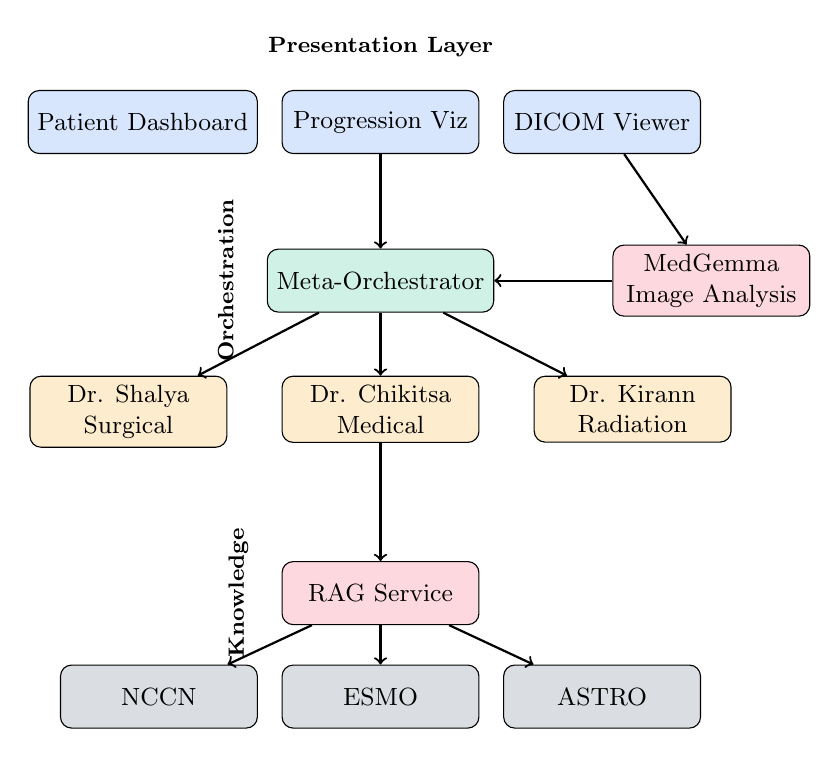
\begin{tikzpicture}[
    node distance=0.8cm,
    box/.style={rectangle, draw, rounded corners, minimum width=2.5cm, minimum height=0.8cm, align=center, font=\small},
    layer/.style={rectangle, draw, dashed, rounded corners, minimum width=7cm, minimum height=2cm},
    arrow/.style={->, thick}
]

% Presentation Layer
\node[box, fill=skyblue!20] (ui) {Patient Dashboard};
\node[box, fill=skyblue!20, right=0.3cm of ui] (viz) {Progression Viz};
\node[box, fill=skyblue!20, right=0.3cm of viz] (dicom) {DICOM Viewer};

% Orchestration Layer
\node[box, fill=emerald!20, below=1.2cm of viz] (orch) {Meta-Orchestrator};
\node[box, fill=amber!20, below left=0.8cm and 0.5cm of orch] (agent1) {Dr. Shalya\\Surgical};
\node[box, fill=amber!20, below=0.8cm of orch] (agent2) {Dr. Chikitsa\\Medical};
\node[box, fill=amber!20, below right=0.8cm and 0.5cm of orch] (agent3) {Dr. Kirann\\Radiation};

% Knowledge Layer
\node[box, fill=rose!20, below=1.5cm of agent2] (rag) {RAG Service};
\node[box, fill=slate!20, below left=0.5cm and 0.3cm of rag] (nccn) {NCCN};
\node[box, fill=slate!20, below=0.5cm of rag] (esmo) {ESMO};
\node[box, fill=slate!20, below right=0.5cm and 0.3cm of rag] (astro) {ASTRO};

% MedGemma
\node[box, fill=rose!20, right=1.5cm of orch] (medgemma) {MedGemma\\Image Analysis};

% Arrows
\draw[arrow] (viz) -- (orch);
\draw[arrow] (orch) -- (agent1);
\draw[arrow] (orch) -- (agent2);
\draw[arrow] (orch) -- (agent3);
\draw[arrow] (agent2) -- (rag);
\draw[arrow] (rag) -- (nccn);
\draw[arrow] (rag) -- (esmo);
\draw[arrow] (rag) -- (astro);
\draw[arrow] (dicom) -- (medgemma);
\draw[arrow] (medgemma) -- (orch);

% Labels
\node[above=0.3cm of viz, font=\footnotesize\bfseries] {Presentation Layer};
\node[left=0.3cm of orch, font=\footnotesize\bfseries, rotate=90, anchor=south] {Orchestration};
\node[left=0.3cm of rag, font=\footnotesize\bfseries, rotate=90, anchor=south] {Knowledge};

\end{tikzpicture}
\caption{High-level system architecture showing the three-layer design with multi-agent orchestration and RAG-grounded knowledge retrieval.}
\label{fig:architecture}
\end{figure}

\subsection{Multi-Agent Orchestration}

Our system employs seven specialist agents, each with a distinct clinical persona and RAG knowledge source:

\begin{table}[H]
\centering
\small
\begin{tabular}{@{}lll@{}}
\toprule
\textbf{Agent} & \textbf{Specialty} & \textbf{RAG Source} \\
\midrule
Dr. Shalya & Surgical Oncology & NCCN \\
Dr. Chikitsa & Medical Oncology & NCCN, ESMO \\
Dr. Kirann & Radiation Oncology & ASTRO \\
Dr. Chitran & Onco-Radiology & ACR \\
Dr. Marga & Pathology & CAP \\
Dr. Anuvamsha & Genetics & ClinVar, CIViC \\
Dr. Shanti & Palliative Care & NCCN Supportive \\
\bottomrule
\end{tabular}
\caption{Specialist agents with their clinical focus and primary RAG knowledge sources.}
\label{tab:agents}
\end{table}

\subsubsection{Chain of Debate Protocol}

Deliberation proceeds through three rounds:

\begin{enumerate}[leftmargin=*]
    \item \textbf{Initial Opinions}: Parallel consultation of relevant specialists
    \item \textbf{Cross-Review}: Agents challenge each other's assumptions
    \item \textbf{Consensus}: Synthesis of recommendations with documented dissent
\end{enumerate}

% Deliberation Flow Diagram
\begin{figure}[H]
\centering
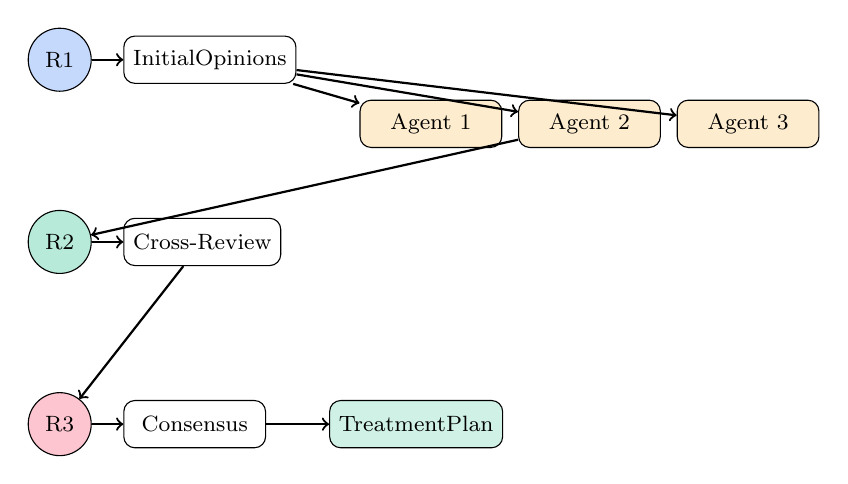
\begin{tikzpicture}[
    node distance=0.6cm,
    round/.style={circle, draw, minimum size=0.8cm, font=\footnotesize},
    box/.style={rectangle, draw, rounded corners, minimum width=1.8cm, minimum height=0.6cm, font=\footnotesize},
    arrow/.style={->, thick}
]

% Round 1
\node[round, fill=skyblue!30] (r1) {R1};
\node[box, right=0.4cm of r1] (r1t) {Initial\\Opinions};
\node[box, fill=amber!20, below right=0.2cm and 0.8cm of r1t] (a1) {Agent 1};
\node[box, fill=amber!20, right=0.2cm of a1] (a2) {Agent 2};
\node[box, fill=amber!20, right=0.2cm of a2] (a3) {Agent 3};

% Round 2
\node[round, fill=emerald!30, below=1.5cm of r1] (r2) {R2};
\node[box, right=0.4cm of r2] (r2t) {Cross-\\Review};

% Round 3
\node[round, fill=rose!30, below=1.5cm of r2] (r3) {R3};
\node[box, right=0.4cm of r3] (r3t) {Consensus};
\node[box, fill=emerald!20, right=0.8cm of r3t] (final) {Treatment\\Plan};

% Arrows
\draw[arrow] (r1) -- (r1t);
\draw[arrow] (r1t) -- (a1);
\draw[arrow] (r1t) -- (a2);
\draw[arrow] (r1t) -- (a3);
\draw[arrow] (a2) -- (r2);
\draw[arrow] (r2) -- (r2t);
\draw[arrow] (r2t) -- (r3);
\draw[arrow] (r3) -- (r3t);
\draw[arrow] (r3t) -- (final);

\end{tikzpicture}
\caption{Chain of Debate deliberation protocol with three rounds.}
\label{fig:deliberation}
\end{figure}

\subsection{MedGemma Integration}

We integrate Google's MedGemma 4B multimodal model for medical image analysis. The integration supports:

\begin{itemize}[leftmargin=*]
    \item DICOM upload with in-browser parsing
    \item Phone camera capture with quality validation
    \item Gallery upload for existing photos
    \item Automated finding extraction and measurement
\end{itemize}

\subsubsection{Image Preprocessing Pipeline}

For DICOM inputs, we apply windowing transformations appropriate to the imaging modality (lung, bone, soft tissue presets for CT). For phone-captured images, we perform:

\begin{enumerate}[leftmargin=*]
    \item Grayscale conversion
    \item Perspective correction
    \item Histogram equalization
    \item Glare removal
    \item Automatic inversion detection
\end{enumerate}

\section{Progressive Disclosure Visualization}

\subsection{Design Principles}

Our visualization framework is grounded in established HCI principles \cite{saloni2025,cogload2020}:

\begin{enumerate}[leftmargin=*]
    \item \textbf{Progressive Disclosure}: Show complexity only when needed
    \item \textbf{Semantic Color Mapping}: Red=progression/bad, Green/Blue=response/good
    \item \textbf{Direct Labeling}: Labels on data, not in separate legends
    \item \textbf{Gestalt Grouping}: Use proximity and similarity for intuitive organization
    \item \textbf{Preattentive Processing}: Leverage size, color, position for instant recognition
\end{enumerate}

\subsection{Four-Level Expertise Adaptation}

We identified four distinct user personas with different information needs:

% User Levels Table
\begin{table}[H]
\centering
\small
\begin{tabular}{@{}p{1.5cm}p{2.5cm}p{2.5cm}@{}}
\toprule
\textbf{Level} & \textbf{User} & \textbf{Information Need} \\
\midrule
1 & Patient/Caregiver & ``Is it getting better or worse?'' \\
2 & Non-oncologist Clinician & Clinical summary, action items \\
3 & Oncologist & RECIST details, treatment response \\
4 & Radiologist & Full measurements, technical detail \\
\bottomrule
\end{tabular}
\caption{Four expertise levels with corresponding information needs.}
\label{tab:levels}
\end{table}

\subsubsection{Level 1: Patient/Caregiver View}

The patient view employs a ``traffic light'' metaphor for immediate comprehension:

\begin{itemize}[leftmargin=*]
    \item \textcolor{emerald}{\textbf{Green}}: Excellent response (CR) or good response (PR)
    \item \textcolor{amber}{\textbf{Yellow}}: Stable disease (SD)
    \item \textcolor{rose}{\textbf{Red}}: Progression requiring attention (PD)
\end{itemize}

Plain language explanations accompany each status, with optional expanded detail. A simplified ``journey timeline'' shows relative tumor burden over time using proportionally-sized circles.

\subsubsection{Level 2: Non-Oncologist Clinician View}

This level adds:
\begin{itemize}[leftmargin=*]
    \item Numeric percent change from baseline
    \item Key metrics (baseline sum, current sum, nadir)
    \item Waterfall chart showing change magnitude
    \item Suggested clinical actions based on response
\end{itemize}

\subsubsection{Level 3: Oncologist View}

Full RECIST 1.1 details including:
\begin{itemize}[leftmargin=*]
    \item Individual target lesion measurements
    \item Spider plot showing per-lesion trajectories
    \item Response reasoning with threshold references
    \item New lesion and non-target progression flags
\end{itemize}

\subsubsection{Level 4: Radiologist/Expert View}

Complete technical detail:
\begin{itemize}[leftmargin=*]
    \item Full measurement matrix across all timepoints
    \item Study comparison tools
    \item Assessment history table
    \item DICOM metadata and study UIDs
\end{itemize}

% Progressive Disclosure Diagram
\begin{figure}[H]
\centering
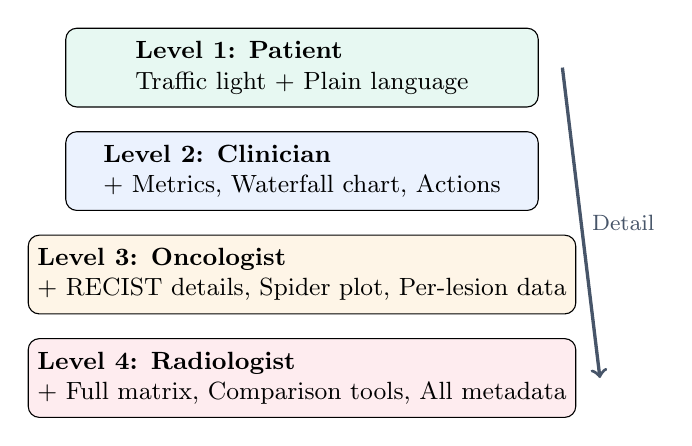
\begin{tikzpicture}[
    node distance=0.4cm,
    level/.style={rectangle, draw, rounded corners, minimum width=6cm, minimum height=1cm, align=left, font=\small}
]

\node[level, fill=emerald!10] (l1) {
    \textbf{Level 1: Patient} \\
    Traffic light + Plain language
};

\node[level, fill=skyblue!10, below=0.3cm of l1] (l2) {
    \textbf{Level 2: Clinician} \\
    + Metrics, Waterfall chart, Actions
};

\node[level, fill=amber!10, below=0.3cm of l2] (l3) {
    \textbf{Level 3: Oncologist} \\
    + RECIST details, Spider plot, Per-lesion data
};

\node[level, fill=rose!10, below=0.3cm of l3] (l4) {
    \textbf{Level 4: Radiologist} \\
    + Full matrix, Comparison tools, All metadata
};

% Arrow showing increasing detail
\draw[->, very thick, slate] ($(l1.east)+(0.3,0)$) -- ($(l4.east)+(0.3,0)$) node[midway, right, font=\footnotesize] {Detail};

\end{tikzpicture}
\caption{Progressive disclosure hierarchy showing increasing detail across expertise levels.}
\label{fig:progressive}
\end{figure}

\subsection{Interactive Chart Modalities}

\subsubsection{Tumor Burden Waterfall Chart}

Displays percent change from baseline for each target lesion, sorted by response magnitude. RECIST threshold lines (-30\% for PR, +20\% for PD) provide immediate context. Color encoding:
\begin{itemize}[leftmargin=*]
    \item \textcolor{emerald}{Emerald}: $\leq$-30\% (PR achieved)
    \item \textcolor{skyblue}{Blue}: Shrinking (<0\%)
    \item \textcolor{amber}{Yellow}: Stable (0-20\%)
    \item \textcolor{rose}{Red}: Growing ($\geq$20\%)
\end{itemize}

\subsubsection{Swimmer Plot}

Horizontal timeline showing response status over weeks from baseline. Each segment is colored by RECIST response category, with markers at assessment timepoints. This visualization is commonly used in oncology clinical trial publications.

\subsubsection{Spider Plot}

Line chart showing individual lesion trajectories as percent change from baseline over time. Enables identification of differential response patterns (e.g., one lesion progressing while others respond).

\subsubsection{Anatomical Heat Map}

Body silhouette with positioned markers representing lesion locations. Marker size encodes current tumor size; color encodes response status. Provides anatomical context lacking in tabular data.

\subsubsection{Response Donut}

Proportional visualization showing distribution of lesions across response categories. Center displays total lesion count.

\section{RECIST 1.1 Implementation}

\subsection{Algorithm}

We implement the Response Evaluation Criteria in Solid Tumors (RECIST) version 1.1 \cite{recist2009}:

\begin{algorithm}[H]
\caption{RECIST 1.1 Response Calculation}
\begin{algorithmic}[1]
\Require Target lesions $L$, current measurements $M_c$, baseline measurements $M_b$
\State $S_b \gets \sum_{l \in L} diameter(M_b[l])$
\State $S_c \gets \sum_{l \in L} diameter(M_c[l])$
\State $S_{nadir} \gets \min(\{S_t : t \in timepoints\})$
\State $\Delta_b \gets (S_c - S_b) / S_b \times 100$
\State $\Delta_n \gets (S_c - S_{nadir}) / S_{nadir} \times 100$
\If{all lesions disappeared}
    \State \Return CR
\ElsIf{$\Delta_b \leq -30$}
    \State \Return PR
\ElsIf{$\Delta_n \geq 20$ \textbf{and} $S_c - S_{nadir} \geq 5$mm}
    \State \Return PD
\Else
    \State \Return SD
\EndIf
\end{algorithmic}
\end{algorithm}

\subsection{Handling Special Cases}

\begin{itemize}[leftmargin=*]
    \item \textbf{Lymph nodes}: Use short axis for measurement; CR requires <10mm
    \item \textbf{New lesions}: Automatic PD regardless of target lesion response
    \item \textbf{Non-target progression}: Unequivocal progression triggers PD
    \item \textbf{Not evaluable}: Missing measurements or imaging quality issues
\end{itemize}

\section{Implementation Details}

\subsection{Technology Stack}

\begin{itemize}[leftmargin=*]
    \item \textbf{Frontend}: Next.js 15, React 19, Tailwind CSS, shadcn/ui
    \item \textbf{Visualization}: Custom SVG/Canvas components
    \item \textbf{DICOM}: dicom-parser (client-side), Cornerstone.js
    \item \textbf{AI}: Claude 3.5 (orchestration), MedGemma 4B (imaging)
    \item \textbf{RAG}: Gemini File Search API
    \item \textbf{Storage}: IndexedDB (client), Cloudflare R2 (optional server)
\end{itemize}

\subsection{Component Architecture}

Key visualization components:

\begin{lstlisting}[language=Java, basicstyle=\ttfamily\tiny]
components/my-imaging/
  DiseaseProgressionViz.tsx  // Main 4-level component
  InteractiveProgressionCharts.tsx
    TumorBurdenWaterfall   // Waterfall chart
    SwimmerPlot            // Timeline view  
    AnatomicalHeatMap      // Body map
    ResponseDonut          // Proportions
    SpiderPlot             // Lesion trajectories
  ProgressionTimeline.tsx   // Legacy timeline
\end{lstlisting}

\subsection{Performance Considerations}

\begin{itemize}[leftmargin=*]
    \item DICOM parsing performed client-side to avoid upload latency
    \item Images cached in IndexedDB for offline access
    \item Lazy loading of detailed views to minimize initial render
    \item Debounced hover states to reduce re-renders
\end{itemize}

\section{Discussion}

\subsection{Design Tradeoffs}

\subsubsection{Simplicity vs. Completeness}

The four-level progressive disclosure balances the need for simplicity (patients) with completeness (radiologists). Users can access appropriate detail without cognitive overload.

\subsubsection{Automation vs. Control}

MedGemma provides automated measurements, but clinicians can override and manually adjust. The system functions as decision support, not autonomous diagnosis.

\subsubsection{Privacy vs. Convenience}

Client-side processing enables privacy-preserving analysis, but limits model size. Server-side options available for institutions with appropriate infrastructure.

\subsection{Limitations}

\begin{enumerate}[leftmargin=*]
    \item MedGemma accuracy on phone-captured images requires validation
    \item Multi-agent deliberation latency (~30 seconds) may not suit urgent cases
    \item RECIST requires manual confirmation of target lesion correspondence across timepoints
    \item System requires internet connectivity for AI features
\end{enumerate}

\subsection{Future Work}

\begin{enumerate}[leftmargin=*]
    \item Volumetric RECIST (vRECIST) implementation
    \item Integration with hospital PACS systems
    \item Multilingual support for Indian languages
    \item Clinical validation studies
    \item Mobile-native application
\end{enumerate}

\section{Conclusion}

We presented an open-source AI-augmented Virtual Tumor Board system with novel progressive disclosure visualizations for disease progression monitoring. By adapting information density to user expertise levels, our system reduces cognitive load while maintaining clinical accuracy. The integration of multi-agent deliberation with MedGemma imaging analysis provides comprehensive decision support previously available only through commercial solutions. Our work demonstrates that thoughtful human-centered design can democratize access to expert oncology care, particularly benefiting resource-limited healthcare settings.

\section*{Acknowledgments}

We thank the open-source community for foundational libraries including dicom-parser, Cornerstone.js, and the Gemini team for MedGemma. Visualization principles were informed by Saloni Dattani's guide to data visualization.

\section*{Code Availability}

Source code is available at: \url{https://github.com/oss-virtual-tumor-board}

% References
\begin{thebibliography}{99}

\bibitem{navify2024}
Roche Diagnostics. NAVIFY Clinical Hub for Tumor Boards. 2024.

\bibitem{maidxo2025}
Microsoft Research. MAI-DxO: Multi-Agent Diagnostic Orchestrator. Sequential Diagnosis with Language Models. 2025.

\bibitem{medgemma2025}
Google Health. MedGemma: Open Models for Medical Image and Text Understanding. 2025.

\bibitem{saloni2025}
Dattani S. Saloni's Guide to Data Visualization. Scientific Discovery. December 2025.

\bibitem{cogload2020}
Sweller J, van Merrienboer JJG, Paas F. Cognitive Architecture and Instructional Design: 20 Years Later. Educational Psychology Review. 2020.

\bibitem{recist2009}
Eisenhauer EA, et al. New response evaluation criteria in solid tumours: Revised RECIST guideline (version 1.1). European Journal of Cancer. 2009;45(2):228-247.

\bibitem{nlptb2023}
Various Authors. Natural Language Processing for Tumor Board Documentation. Journal of Clinical Oncology Informatics. 2023.

\bibitem{mlonc2024}
Various Authors. Machine Learning Approaches for Cancer Treatment Recommendation. npj Digital Medicine. 2024.

\end{thebibliography}

% Appendix
\appendix

\section{Agent System Prompts}

\subsection{Dr. Chitran (Onco-Radiologist)}

\begin{lstlisting}[basicstyle=\ttfamily\tiny, breaklines=true]
You are Dr. Chitran, an Oncologic Radiologist 
interpreting imaging for staging, response 
assessment, and surveillance.

Your evaluation framework:
1. STAGING IMAGING: Is staging complete?
2. REPORT REVIEW: Key findings, measurements
3. RESPONSE ASSESSMENT: Per RECIST 1.1
4. ANATOMIC DETAIL: Surgical planning
5. SUSPICIOUS FINDINGS: Biopsy targets
6. FOLLOW-UP: Surveillance protocol

Primary guideline: ACR Appropriateness Criteria
\end{lstlisting}

\section{RECIST 1.1 Response Criteria}

\begin{table}[H]
\centering
\small
\begin{tabular}{@{}lp{5cm}@{}}
\toprule
\textbf{Response} & \textbf{Criteria} \\
\midrule
CR & Disappearance of all target lesions; lymph nodes <10mm short axis \\
PR & $\geq$30\% decrease in sum of diameters from baseline \\
PD & $\geq$20\% increase from nadir AND $\geq$5mm absolute increase; OR new lesions \\
SD & Neither PR nor PD criteria met \\
\bottomrule
\end{tabular}
\caption{RECIST 1.1 response category definitions.}
\end{table}

\section{Color Semantics}

\begin{table}[H]
\centering
\small
\begin{tabular}{@{}lll@{}}
\toprule
\textbf{Color} & \textbf{Meaning} & \textbf{Hex} \\
\midrule
\textcolor{emerald}{Emerald} & Excellent (CR) & \#10b981 \\
\textcolor{skyblue}{Blue} & Good (PR) & \#3b82f6 \\
\textcolor{amber}{Yellow} & Stable (SD) & \#eab308 \\
\textcolor{rose}{Red} & Progression (PD) & \#ef4444 \\
\textcolor{slate}{Gray} & Not evaluable & \#64748b \\
\bottomrule
\end{tabular}
\caption{Semantic color mapping for response visualization.}
\end{table}

\end{document}
